% !TeX program = xelatex
\documentclass[handout,defaultFootings,slideTotalNumber,ENlocalization,lightTitle,hideSidebar,classicFont]{mul-beamer}
\usepackage{fontspec}
\usepackage{booktabs}
\usepackage{tikz}
\usetikzlibrary{arrows.meta,positioning}
\setsansfont{Noto Sans CJK SC}
\XeTeXlinebreaklocale "zh"
\XeTeXlinebreakskip=0pt plus 1pt
\definecolor{ink}{HTML}{23373B}
\definecolor{paper}{HTML}{FAFAF7}
\definecolor{teal}{HTML}{116D68}
\definecolor{amber}{HTML}{D28228}
\setbeamertemplate{navigation symbols}{}
\setlength{\parskip}{3pt}
\graphicspath{{figures/}}
\renewcommand{\funneldisplay}{\sffamily}
\setbeamerfont{frametitle}{size=\large,series=\bfseries}
\setSlogan{}
\conference{从跑者训练日志到可穿戴生理时序}
\newcommand{\credit}[1]{\par\vspace{2pt}{\scriptsize\color{ink!75}#1}\par}
\newcommand{\point}[2]{\par\textcolor{teal}{\textbf{#1}}\par #2\par\vspace{3pt}}
\newcommand{\talk}[2]{\note{#1\par #2}}
\newcommand{\paperone}{Xie, Hao \& Xie, Frontiers in Public Health (2025). \href{https://doi.org/10.3389/fpubh.2025.1647200}{10.3389/fpubh.2025.1647200}}
\newcommand{\papertwo}{Xie, Hao \& Xie, Computational Statistics (2026). \href{https://doi.org/10.1007/s00180-026-01760-4}{10.1007/s00180-026-01760-4}}
\newcommand{\nolte}{Nolte, S. (2024). \textit{More Than Just Associations: An Introduction to Causal Inference for Sport Science}. 硕士论文，德国科隆体育大学。}
\tikzset{factor/.style={draw=teal!60,fill=teal!7,rounded corners=2pt,inner sep=6pt,align=center},patharrow/.style={-{Stealth},semithick,draw=teal}}
\title{运动损伤与康复的因果推断}
\subtitle{从跑者训练日志到可穿戴生理时序}
\author{谢淘}
\institute[高校教师岗位科研汇报]{韩国庆一大学体育训练博士阶段｜高校教师岗位科研汇报}
\date{}
% To show speaker notes, uncomment the following line and recompile.
% \setbeameroption{show notes}
\begin{document}
\begin{frame}
\titlepage
\end{frame}

\begin{frame}{汇报目录}
\tableofcontents
\end{frame}


\section{研究现状}\subsection{当前研究背景}

\begin{frame}{研究背景｜运动损伤文献中，关联词比因果词更常见}
\begin{columns}[c,onlytextwidth]
\column{.44\textwidth}
\point{五年文献分布}{限定运动损伤精确词组时，关联词命中 341 篇次，因果词命中 7 篇次。放宽到含 sports 的检索后，两者相差仍大。}
\point{怎么理解约 2\%？}{每 100 个关联词命中，对应约 2 个因果词命中。宽泛口径为 2.20\%，精确口径为 2.05\%。}
\column{.54\textwidth}\centering
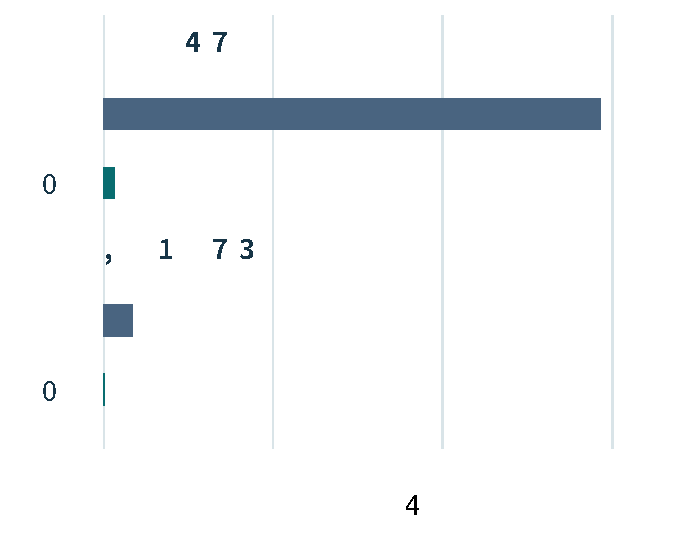
\includegraphics[width=\linewidth]{pubmed-total.pdf}
\end{columns}
\credit{PubMed 题名／摘要，2021–2025。比值为因果词命中数除以关联词命中数；检索集合可重叠，实际采用的方法需逐篇判读。}
\end{frame}

\subsection{现有研究的局限性}
\begin{frame}{研究缺口｜因果词命中增加，损伤专项研究仍少见}
\begin{columns}[c,onlytextwidth]
\column{.44\textwidth}
\point{从发文趋势看}{宽泛口径从每年 15 篇次升至 36 篇次，最近两年持平。限定损伤词组后，各年只有 0–3 篇次。}
\point{从训练决策看}{既往伤病影响训练安排，早期疼痛也会使运动员主动减量。即使观察到跑量与损伤相关，教练仍需知道：在恢复状况相近时，调整冲刺负荷会怎样改变后续损伤风险？}
\column{.54\textwidth}\centering
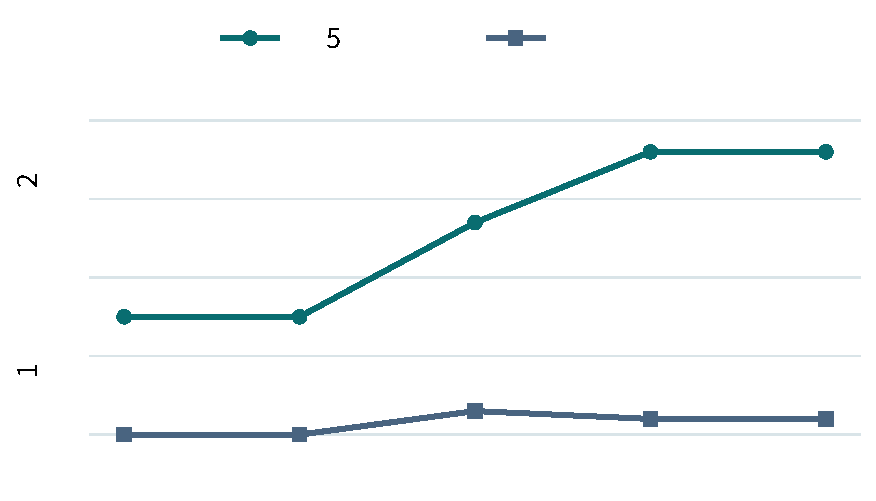
\includegraphics[width=\linewidth]{pubmed-trend.pdf}
\end{columns}
\credit{PubMed 年度导出，2021–2025；精确因果词组在 2021、2022 年无记录。研究问题参照 Nielsen 等（2020）与 Meeuwisse 等（2007）的动态损伤模型。}
\end{frame}

\section{研究必要性}

\begin{frame}{相关不代表因果｜超马补给与完赛表现}
\centering
\begin{tikzpicture}[font=\small]
\node[factor] (e) at (0,1.5){参赛经验};
\node[factor] (n) at (-3.6,0){赛中营养摄入};
\node[factor] (t) at (0,0){训练};
\node[factor] (p) at (2.2,0){赛前能力};
\node[factor] (o) at (4.5,0){比赛表现};
\draw[patharrow](e)--(n);\draw[patharrow](e)--(t);\draw[patharrow](t)--(p);\draw[patharrow](p)--(o);
\draw[patharrow](n) to[bend right=22] (o);
\end{tikzpicture}
\raggedright\point{一个可检验的解释}{经验丰富者可能更擅长补给，也有更充分的训练。两条路径同时产生摄入与成绩的关联。}
\point{怎样设计比较？}{在该图成立时，按经验调整可阻断这条后门路径。若训练也影响补给，调整集需要重审。}
\credit{据 Simon Nolte (2024)，More Than Just Associations，§4.2，图 8，正文 p. 18 简化重绘。}
\end{frame}


\section{参加的科研项目与学术交流}

\begin{frame}{科研协作与学术交流｜从足球伤例到穿戴数据}
\small
\point{庆一大学博士阶段参与经历（据本人简历）}{青少年足球成熟度与损伤：参与数据整理分析。实时动作纠正强化学习反馈：整理穿戴数据与特征。初中足球外侧踝扭伤：梳理风险因素和研究资料。}
\point{研究方案交流}{与德国科隆体育大学 Simon Nolte 就跑者损伤、跑量与强度的研究设计交流，并征询方法意见。}
\point{学术活动}{2025.12.12 运动康复医学系学术节，关注足球损伤与踝关节不稳。2026.07.16 OpenSim 专题讲座，学习肌骨建模。}
\credit{身份与分工按简历中的参与、交流、参会记录列示。}
\end{frame}


\section{研究成果}

\begin{frame}{科研成果总览｜1–3}
\small\raggedright
{\color{teal}\bfseries 1. Xie T, et al. A causal inference method for athletic injuries based on quantile threshold functions and latent Gaussian DAG models.}\par
Frontiers in Public Health, 2025, 13:1647200. 第一作者、通讯作者｜已发表 DOI: 10.3389/fpubh.2025.1647200\par\medskip
{\color{teal}\bfseries 2. Xie T, et al. Iterative causal discovery uncovers dynamic effects in wearable exercise data.}\par
Computational Statistics, 2026, 41:83. 共同第一作者（署名第1）、通讯作者｜已发表 DOI: 10.1007/s00180-026-01760-4\par\medskip
{\color{teal}\bfseries 3. Xie T, et al. Uncovering the Causal Effects of Injuries on Runners’ Training Through DAG-Guided Mediation Analysis.}\par
BMC Sports Science, Medicine and Rehabilitation. 第一作者｜在审\par\medskip
\end{frame}
\begin{frame}{科研成果总览｜4–6}
\small\raggedright
{\color{teal}\bfseries 4. Xie T, et al. Expected Goals Prediction in Football—A Comparative Study Using Machine Learning Algorithms.}\par
Sports. 第一作者｜在审\par\medskip
{\color{teal}\bfseries 5. Xie T, et al. Application of the Apriori Algorithm in Soccer Games.}\par
AAIA 2023, pp. 54–59. ACM. 第一作者｜会议论文 DOI: 10.1145/3603273.3631190\par\medskip
{\color{teal}\bfseries 6. 基于数据挖掘视角下足球比赛进攻模式研究［硕士学位论文］。}\par
沈阳体育学院，2018。\par\medskip
\end{frame}


\begin{frame}{代表作一｜从损伤日志到有序因果效应}
\begin{center}\begin{tikzpicture}[font=\small,node distance=0.40cm]
\node[factor](n0){损伤数据};
\node[factor,right=of n0](n1){QTF 有序化};\draw[patharrow](n0)--(n1);
\node[factor,right=of n1](n2){OSEM 学习图};\draw[patharrow](n1)--(n2);
\node[factor,right=of n2](n3){OCE 估计};\draw[patharrow](n2)--(n3);
\end{tikzpicture}\end{center}\point{方法创新}{用核密度与分位数阈值把连续训练指标转换成有序等级，结合潜在高斯 DAG 与干预算子，比较等级转换的损伤概率差。}
\point{结构结果}{三条直接候选路径涉及冲刺跑量、主观恢复、主观训练成效。总跑量经训练频次与恢复、力量训练经主观训练成效间接连接损伤。}
\credit{\paperone；第一作者、通讯作者，承担构思、数据整理和初稿。}
\end{frame}


\begin{frame}{研究结果一｜低到中、高等级的转换更值得追踪}
\begin{columns}[T,onlytextwidth]
\column{.55\textwidth}
\centering
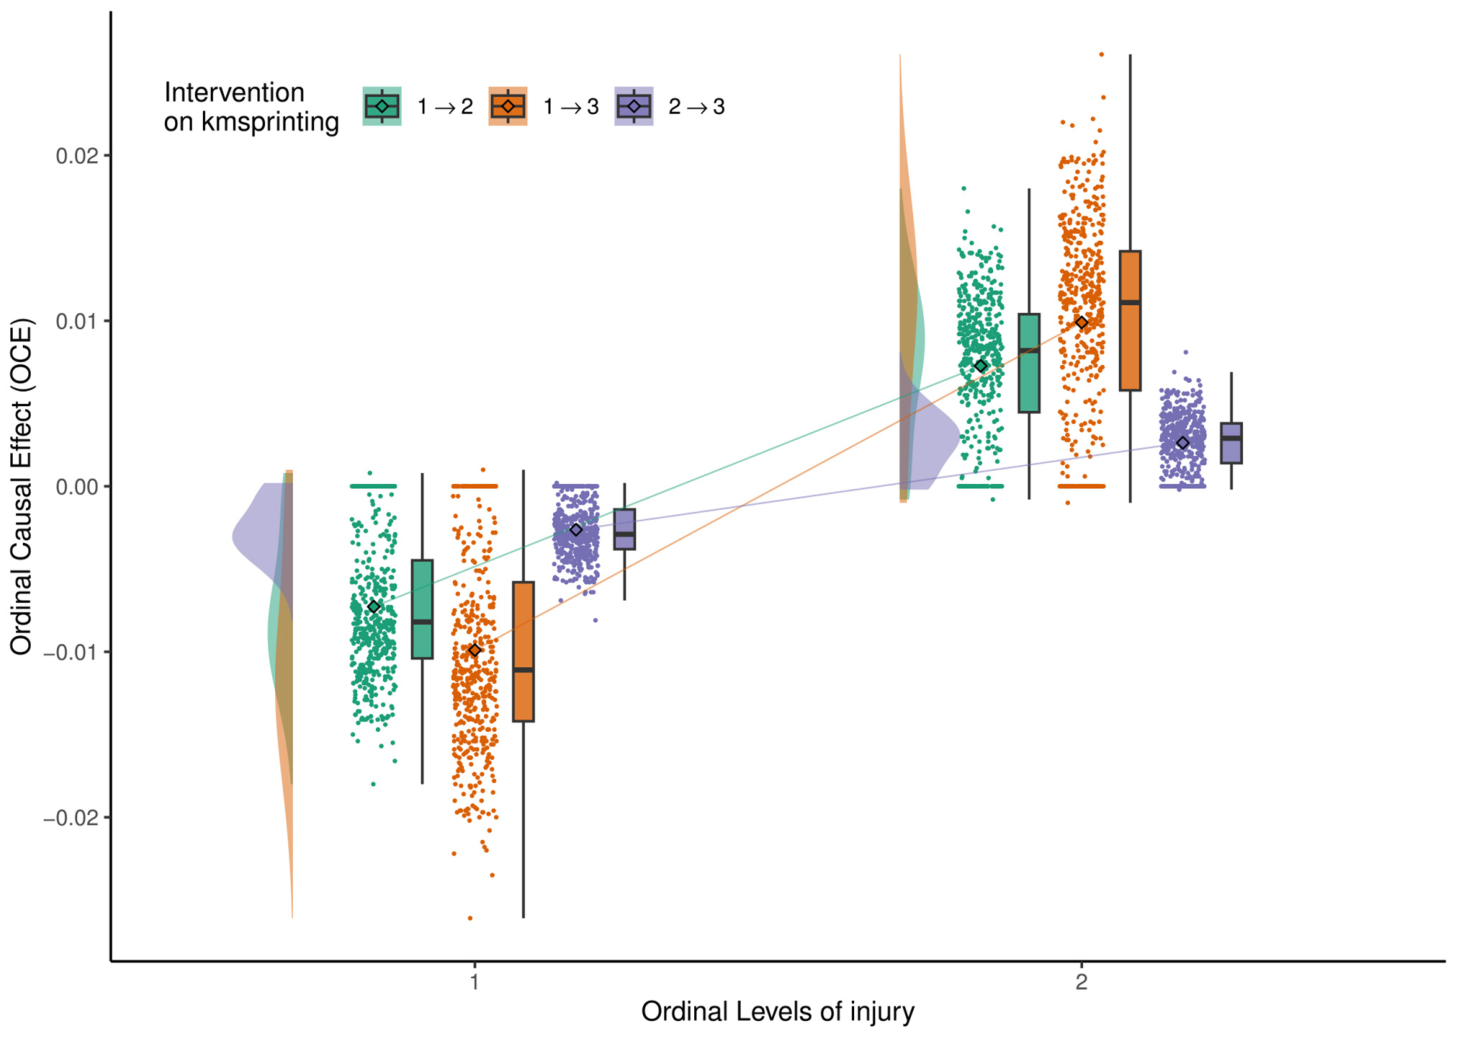
\includegraphics[width=\linewidth,height=.62\textheight,keepaspectratio]{oce.png}
\credit{原论文图 5｜冲刺跑量等级变化的有序效应估计。}
\column{.41\textwidth}
\point{读图}{看 \texttt{Injury = 2}（受伤）对应的分布。正值表示模型估计的损伤概率上升。}
\point{结果}{低 $\to$ 中、低 $\to$ 高时估计偏正；中 $\to$ 高时的估计更接近零。}
\credit{原文 p. 8：“the transition from low to medium intensity (1 → 2) is a critical period for injury risk”}\point{下一步}{用赛季随访明确时间顺序，再检查分级阈值和效应能否迁移。}
\end{columns}
\credit{\paperone · 图 5，CC BY。}

\end{frame}

\begin{frame}{代表作二｜从分钟级序列到时序中介分析}
\begin{center}\begin{tikzpicture}[font=\small,node distance=0.40cm]
\node[factor](n0){穿戴数据};
\node[factor,right=of n0](n1){TS-ICD};\draw[patharrow](n0)--(n1);
\node[factor,right=of n1](n2){候选结构 PAG};\draw[patharrow](n1)--(n2);
\node[factor,right=of n2](n3){中介效应分析};\draw[patharrow](n2)--(n3);
\end{tikzpicture}\end{center}\begin{columns}[T,onlytextwidth]\column{.48\textwidth}\centering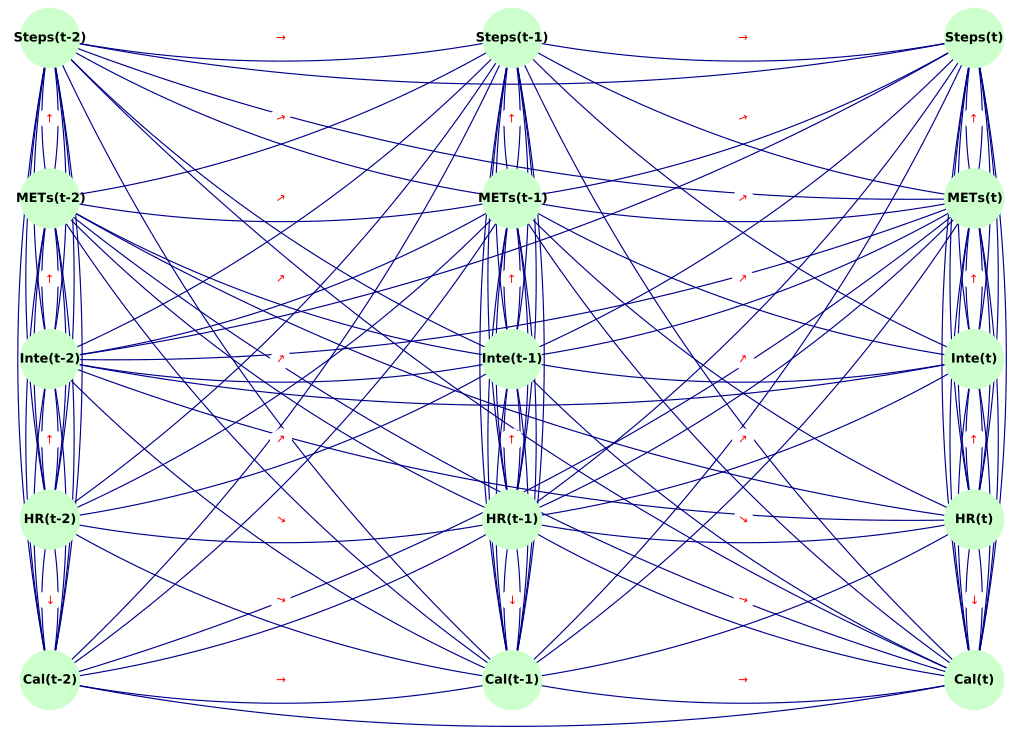
\includegraphics[width=\linewidth,height=.40\textheight,keepaspectratio]{ts-pag.png}
\credit{论文图 7，真实数据的 TS-ICD 输出。}
\column{.49\textwidth}\small
加入时间先后约束，搜索连接过去与当前状态的候选边。论文报告部分祖先图（PAG），部分端点保留方向不确定性。再针对明确路径建立中介模型。\par\medskip
\alert{共同第一作者，署名第 1}，承担研究设计、方法提出、数据分析、制图及撰稿。
\end{columns}\credit{\papertwo，附录图 7，p. 24。}
\end{frame}


\begin{frame}{研究结果二｜强度和步数通过不同路径关联心率}
\begin{columns}[T,onlytextwidth]
\column{.48\textwidth}
\point{滞后强度 → 近期及当前强度 → 心率}{合计间接效应 \alert{11.582}，约占估计总效应的 \alert{73\%}。}
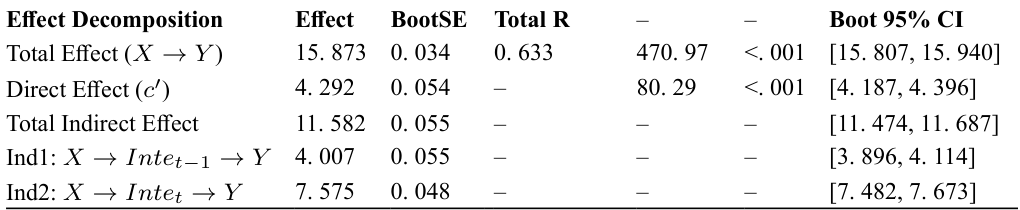
\includegraphics[width=\linewidth]{lagtable.png}
\credit{原论文表 3 · 效应分解节选。}
\column{.48\textwidth}
\point{滞后步数 → 代谢当量（METs）→ 心率}{间接效应 \alert{0.393}（95\% CI 0.389–0.396）；直接效应 $p=0.606$。}
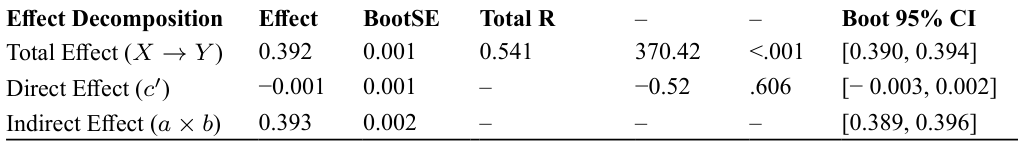
\includegraphics[width=\linewidth]{mettable.png}
\credit{原论文表 4 · 效应分解节选。}
\end{columns}
\begin{alertblock}{结果的适用范围}
330,842 条时间窗观测来自 30 人。估计量依赖模型设定，直接效应未检出；损伤结局有待新队列检验。
\end{alertblock}
\credit{\papertwo}

\end{frame}

\section{未来研究计划}

\begin{frame}{后续研究｜在校园足球中检验负荷与恢复路径}
\point{研究问题}{负荷波动是否经次日恢复与后续损伤相连？该关系在不同队伍、赛季及训练阶段是否稳定？}
\begin{columns}[T,onlytextwidth]
\column{.49\textwidth}
\point{前瞻队列}{基线记录既往损伤与训练水平；每次训练记录时长、主观用力和训练内容；次日随访恢复。条件允许时对设备子样本保留时间戳与处理参数。}
\column{.47\textwidth}
\point{结局与分析}{以每千暴露小时损伤率为主要结局，跟踪踝扭伤与缺训。预设混杂与滞后窗口，按队伍或赛季留出验证，评估校准和路径稳定性。}
\end{columns}
\credit{拟开展研究｜采集前完成伦理审批、知情同意与伤例判定规范。}

\end{frame}

\begin{frame}{研究依据｜青少年足球损伤的观察研究怎样进入实践？}
\point{问题先于模型}{Nielsen 等在运动损伤研究中区分描述、预测与因果目标。开展负荷预警时明确预测窗口；评价预防策略时预先定义可实施的负荷调整。}
\point{足球研究的启示}{Rommers 等在成长中的精英青少年男子足球运动员中，用因果推断框架研究运动能力与损伤，未检出所研究的关联。新队列应同步记录训练暴露、既往伤病与恢复，并验证所选指标。}
\credit{Nielsen et al., BJSM (2020), \href{https://doi.org/10.1136/bjsports-2020-102144}{doi:10.1136/bjsports-2020-102144}；Rommers et al., JSAMS (2021), \href{https://doi.org/10.1016/j.jsams.2021.03.004}{doi:10.1016/j.jsams.2021.03.004}。文献线索来自论文一引文。}
\end{frame}
\begin{frame}{伤后康复｜比较重返赛场策略的收益与风险}
\point{目标试验的设计}{在具备回归专项训练条件的运动员中定义共同起点，比较两种可执行的加量策略。主要结局为复发，辅以功能恢复、缺训天数与回归时间。}
\point{因果分析}{若疼痛或恢复既受前期负荷影响，又决定下一期训练，可预设纵向因果图，用参数 g 公式估计策略下的风险。检查混杂测量、策略重叠和模型设定。}
\point{阶段交付}{第 1 年建立前瞻队列与数据字典；第 2–3 年验证模型；第 4–5 年开展预防或康复试点，将去标识案例用于教学。}
\credit{方法实现：\href{https://github.com/CausalInference/gfoRmula}{gfoRmula}；时序基础：\href{https://github.com/TaoXyjammy/TS-ICD}{TS-ICD}。}
\end{frame}


\begin{frame}{结语｜让训练场上的比较有明确的干预含义}
\point{已完成}{从有序损伤数据估计候选路径，从分钟级穿戴序列解析活动与心率的滞后联系。}
\point{拟开展}{以训练暴露、恢复与后续伤情的前瞻记录，检验校园足球损伤预防和伤后回归策略。}
\bigskip{\Large 感谢各位老师，欢迎提问。}
\end{frame}

\end{document}
